\documentclass{article}
\usepackage{graphicx} % Required for inserting images
\usepackage[top=0.9in, bottom=1in, left=1.5in, right=1.5in]{geometry}
\usepackage[utf8]{inputenc}
\usepackage[icelandic]{babel}
\usepackage[T1]{fontenc}
\usepackage[sc]{mathpazo}
\usepackage[parfill]{parskip}
% Tables and lists
\usepackage{booktabs,tabularx}
\usepackage{multirow}
\usepackage{enumerate}
\usepackage{adjustbox}
\usepackage{multicol}
\usepackage{xcolor}
\usepackage{algpseudocode}
\usepackage{tikz}
\usetikzlibrary{arrows, positioning, calc}

% Math
\usepackage{amsmath, amsfonts, amssymb, amsthm}
% Graphics

\usepackage{graphicx}
\usepackage{tikz}
% Code environment
\usepackage{minted}
%\usepackage{bm}
%\usepackage{siunitx}
%\usepackage{animate}
%\usepackage{hyperref}
%\usepackage{movie15}
%\usepackage{multicol}
%\usepackage{changepage}
\title{Tölvutækni og Forritun Heimadæmi 2}
\author{Ragnar Björn Ingvarsson, rbi3}


\begin{document}
	
	\maketitle
	
	\section{}
	\includegraphics[scale=0.350]{helloworld.png}

	\section{}
	\begin{center}
	\includegraphics[scale=0.200]{stacksmash.png}
	\end{center}
	\begin{itemize}
		\item[a.] Sjáum að ef \textbf{a} er $6$ (fyrsta keyrslan) þá 
			er fylkið nógu stórt til að \texttt{i=8} fer einungis inn 
			á svæði \texttt{d} á hlaðanum en ekki yfir það svo forritið 
			hrynur ekki.
		\item[b.] Hér sést að gildið á \texttt{fun()} breytist ekki þar 
			sem \textbf{d} er á undan \textbf{a} svo við förum strax 
			framhjá svæði \textbf{d} á hlaðanum en forritið hrynur svo 
			þegar það klárar allt svæði \textbf{a}.
		\item[c.] Þegar \textbf{d} er float fær það helminginn af plássi 
			á hlaðanum sem double fær svo forritið hrynur mikið fyrr 
			því það er fljótara að fara yfir svæði \textbf{d}.
	\end{itemize}

	\section{}
	\begin{itemize}
		\item[a.] Fyrst verður \textbf{i} semsagt $4$, síðan bendir 
			\textbf{p} á gildi \textbf{i} og \textbf{q} er svo látið 
			benda á ekkert. \textbf{t} er svo tvöfaldur bendir sem bendir 
			á bendinn \textbf{q} og síðan er látið bendinn sem 
			\textbf{t} bendir á, semsagt \textbf{q}, benda á gildið 
			\textbf{i}. Loks er látið gildið sem \textbf{t} leiðir 
			til, semsagt \textbf{i}, verða $8$.

			Allar breyturnar enda þá á því að enda á $8$.

			\begin{center}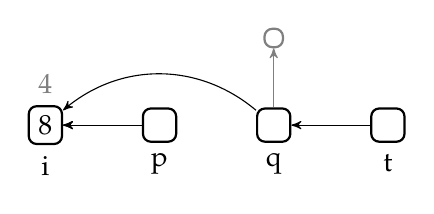
\begin{tikzpicture}[->, >=stealth', cube/.style={rectangle,draw=black, thick, rounded corners=1mm, minimum size=1.2em}]
				\node[cube] (4) {8};
				\node[cube, above=0.01 of 4, draw=white, text=black!50] (8) {4};
				\node[cube, below=0.01 of 4, draw=white] (i) {i};
				\node[cube, right=of 4] (p*) {};
				\node[cube, below=0.01 of p*, draw=white] (p) {p};
				\node[cube, right=of p*] (q*) {};
				\node[cube, below=0.01 of q*, draw=white] (q) {q};
				\node[cube, right=of q*] (t*) {};
				\node[cube, below=0.01 of t*, draw=white] (t) {t};

				\node[cube, above=0.75 of q*, draw=black!50, minimum size=0.01em] (NULL) {};

				\path (p*) edge node {} (4);
				\path (q*) edge[bend right=40] node {} (4);
				\path (q*) edge[draw=black!50] node {} (NULL);
				\path (t*) edge node {} (q*);
				\path (p*) edge node {} (4);

			\end{tikzpicture}
		\end{center}
	\item[b.] Þessar skilgreiningar eru ekki eins vegna þess að í raun 
		virkar hver stjarna bara einu sinni. Þannig að í fyrstu 
		skilgreiningunni erum við að segja að \textbf{p} sé bendir en 
		svo er \textbf{q} bara venjuleg integer tala.

		Hins vegar í seinni skilgreiningunni erum við að segja að 
		\textbf{p} sé bendir og einnig að \textbf{q} sé bendir vegna 
		þess að við skilgreinum aðra stjörnu við \textbf{q}.
	\end{itemize}

	\section{}
	\begin{verbatim}
#include <stdio.h>
#include <stdlib.h>

int min( int a, int b ) {
	return a < b ? a : b;
}
int max( int a, int b ) {
	return a > b ? a : b;
}

int main( int argc, char *argv[] ) {
	int gamer[argc-1];
	for (int i=0; i < argc-1; i++) {
		gamer[i] = atoi(argv[i+1]);
	}
	int l = min(min(gamer[0],gamer[1]),gamer[2]);
	int h = max(max(gamer[0],gamer[1]),gamer[2]);
	int mid = gamer[0] + gamer[1] + gamer[2] - l - h;

	printf("%i\n", mid);
	return 0;
}
	\end{verbatim}
	\includegraphics[scale=0.275]{mid.png}
	\section{}
	\begin{verbatim}
struct Node* vec2list(int a[], int n) {
    struct Node *head, *p;
    int i;
    
    head = NULL;

    /* Þið skrifið þennan hluta */

	struct Node *q;
	for ( i = 0; i < n; i++ ) {
		q = (struct Node*)malloc(sizeof(struct Node));
		q->val = a[i];
		q->next = NULL;

		if (head == NULL) {
			head = q;
		} else {
			p->next = q;
		}
		p = q;
	}
    
    return head;
}

	\end{verbatim}
	\includegraphics[scale=0.275]{linked.png}
	

\end{document}
